\documentclass[10pt,fleqn]{article} % Default font size and left-justified equations
\usepackage[%
    pdftitle={Modélisation SLCI : Rapidité des systèmes},
    pdfauthor={Xavier Pessoles}]{hyperref}
    
\input{style/new_style}
\input{style/macros_SII}
\usepackage{multicol}
\usepackage{siunitx}
%\usepackage{picins}
\fichetrue
%\fichefalse

\proftrue
\proffalse

\tdtrue
%\tdfalse

\courstrue
\coursfalse

\def\discipline{Sciences \\Industrielles de \\ l'Ingénieur}
\def\xxtete{Sciences Industrielles de l'Ingénieur}

\def\classe{PTSI}
\def\xxnumpartie{Cycle 02}
\def\xxpartie{Modéliser les systèmes asservis }


\def\xxnumchapitre{}%Chapitre 3 \vspace{.2cm}}
\def\xxchapitre{}%\hspace{.12cm} Précision des systèmes}


\def\xxtitreexo{Conception de la commande d’un robot chirurgical}
\def\xxsourceexo{\hspace{.2cm} \footnotesize{Centrale Supelec PSI --  2015}}


\def\xxposongletx{2}
\def\xxposonglettext{1.45}
\def\xxposonglety{20}
%\def\xxonglet{Part. 1 -- Ch. 3}
\def\xxonglet{Cycle 02}

\def\xxactivite{Colle  03}
\def\xxauteur{\textsl{Xavier Pessoles}}

\def\xxcompetences{%
\textsl{%
\textbf{Savoirs et compétences :}\\
%Les sources sont associées par un \emph{hacheur série}. La détermination des grandeurs électriques associées à ce montage permet de conclure vis à vis du cahier des charges.
%\noindent \textbf{Résoudre :} à partir des modèles retenus :
%\begin{itemize}[label=\ding{112},font=\color{ocre}] 
%\item choisir une méthode de résolution analytique, graphique, numérique;
%\item mettre en \oe{}uvre une méthode de résolution.
%\end{itemize}
%\begin{itemize}[label=\ding{112},font=\color{ocre}] 
%\item \textit{Rés -- C1.1 :} Loi entrée sortie géométrique et cinématique -- Fermeture géométrique.
%\end{itemize}
%
%\noindent \textit{Mod2 -- C4.1 :} Représentation par schéma bloc.
}}

\def\xxfigures{
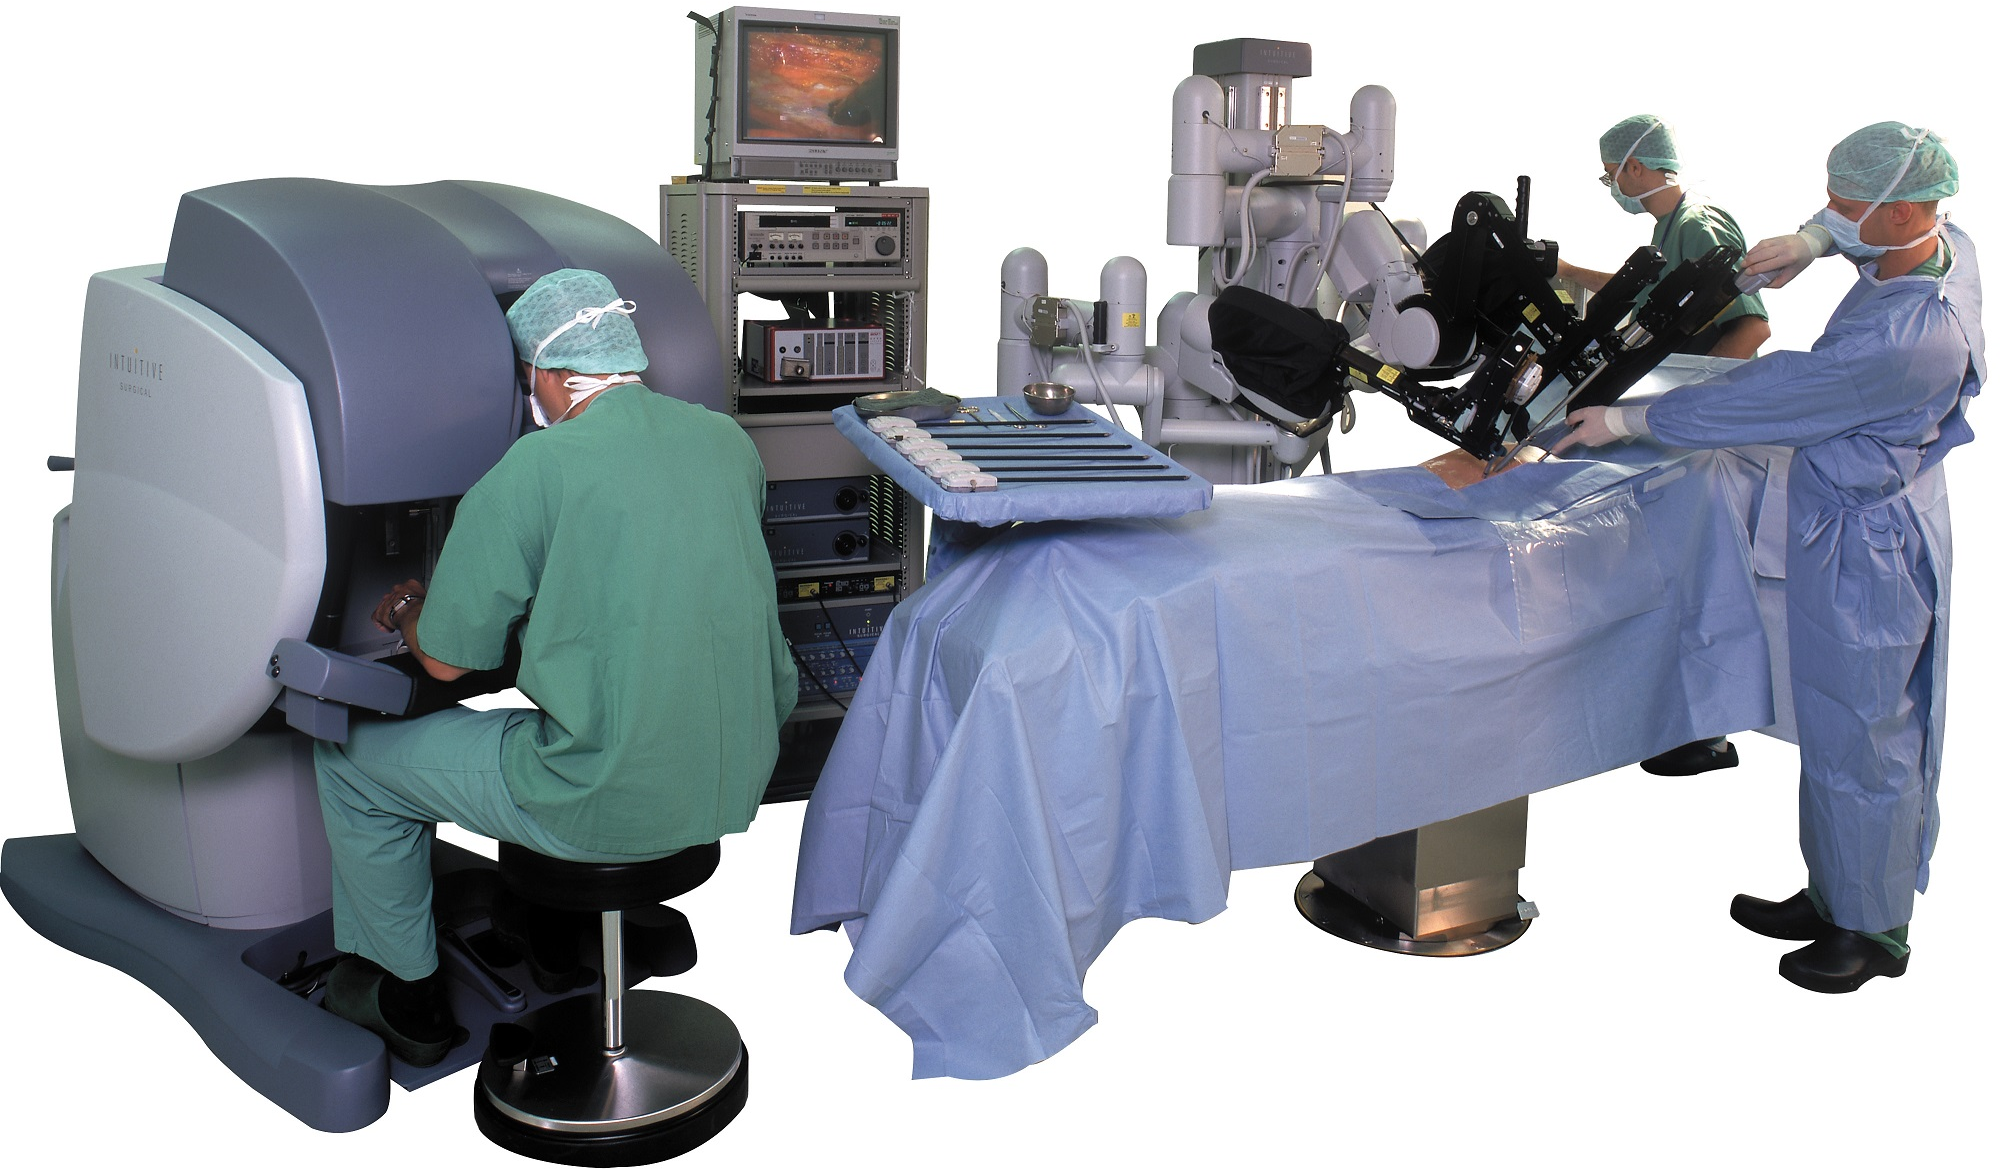
\includegraphics[width=.6\linewidth]{images/fig_01}
}%figues de la page de garde


\def\xxpied{%
Cycle 02 -- Modéliser les SLCI afin de prévoir leur comportement\\
%Chapitre 3 -- \xxactivite%
}

\setcounter{secnumdepth}{5}
%---------------------------------------------------------------------------

\usepackage{pgfplots}
\begin{document}

%\chapterimage{png/Fond_Cin}
\input{style/new_pagegarde}
\vspace{4.5cm}
\pagestyle{fancy}
\thispagestyle{plain}

\def\columnseprulecolor{\color{ocre}}
\setlength{\columnseprule}{0.4pt} 

\def\pathfig{images}

\begin{multicols}{2}



%\section{Fauteuil dynamique de cinéma}
\subsection*{Présentation du système}
\ifprof
\else
Afin d’améliorer les conditions d’opérations chirurgicales dites mini invasives (comme la précision d’opération
et le confort du chirurgien), des robots chirurgicaux ont vu le jour. Cette étude s’intéresse à l’un d’entre eux : le
robot Da Vinci. Le chirurgien peut atteindre sa cible grâce à des outils longs et fins traversant le patient grâce
à une incision de l’ordre du centimètre.


Le système étudié est composé de deux sous-systèmes principaux :
\begin{itemize}
\item l’ensemble \{console de commande + bras maîtres\} permet au chirurgien de visualiser et de commander les
mouvements des outils adéquats à l’intérieur du patient via une caméra haute définition dont l’image est
retransmise par l’intermédiaire d’écrans. Le chirurgien commande les mouvements des outils grâce à deux
bras maîtres dont les extrémités sont maintenues dans chaque main ;
\item les bras esclaves reçoivent les consignes issues du chirurgien par l’intermédiaire des bras maîtres. Il y a au
total 3 bras esclaves : deux manipulent chacun un outil, le troisième manipule une caméra.
\end{itemize}
\begin{center}
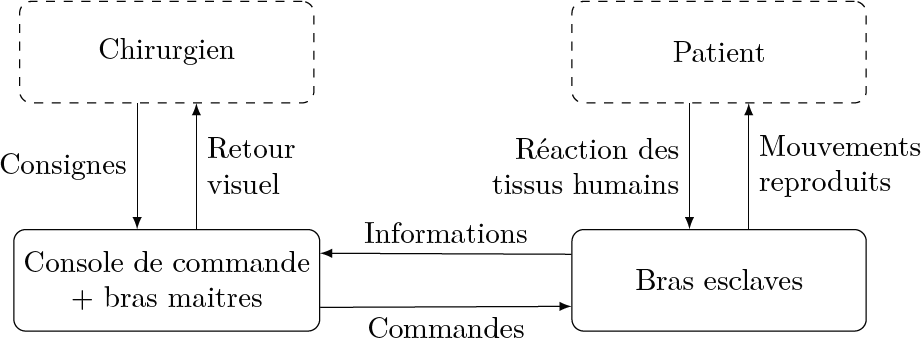
\includegraphics[width=\linewidth]{images/fig_02}
%\textit{}
\end{center}

Le mouvement de l'axe 1 est régi par l'équation suivante : 
$\Delta C_1(t)=J\dfrac{\dd^2 \Delta \theta_1(t)}{\dd t^2} - k_1 \dfrac{r_9'}{r_0}h_2 \Delta F_x(t)$ avec $J=\SI{1,98e-5}{kg.m^2}$, $k_1\dfrac{r_9'}{r_0}=0,00717$, $h_2=\SI{0,2}{m}$.

Le couple moteur $\Delta C_1(t)$ est fourni par une machine à courant continu modélisée par les équations suivantes : 
$u_1(t)=L\dfrac{\dd i_1(t)}{\dd t}  + Ri_1(t)+e_1(t)$, $e_1(t)=k_e \dfrac{\dd \Delta \theta_1(t)}{\dd t}$, $\Delta C_1(t) = k_t i_1(t)$ avec $u_1(t)$ la tension aux bornes du moteur, $i_1(t)$ l’intensité traversant le moteur et $e_1(t)$ la force contre
électromotrice, avec $R=\SI{2,08}{\Omega}$, $k_t = \SI{0,0525}{N.m.A^{-1}}$ et $k_e = \SI{0,0525}{V.s.rad^{-1}}$.

On fait l’hypothèse que l’influence de l’inductance $L$ est négligeable sur les performances attendues, soit $L=0$.

La consigne est notée $\Delta \theta _{c1}(t)$. Le cahier des charges sélectif conduit à choisir un correcteur associant une anticipation (via la présence de $\sigma_4$ dans la relation suivante) et une correction PID. La tension de commande du moteur est donnée par : $U_1(p)=\left( \Delta \theta_{c1}(p)-\Delta \theta_1(p)\right) \left(\sigma_1 + \dfrac{\sigma_2}{p}\right)- \sigma_3p \Delta \theta_1(p)+\sigma_4\Delta \theta_{c1}(p)$
avec $\Delta \theta_{c1}(p)$ la consigne de position angulaire exprimée dans le domaine symbolique.

\subparagraph{}\textit{Compléter le schéma-blocs.}
\ifprof
\begin{corrige}
\end{corrige}
\else
\fi

Pour la suite, on considère la perturbation nulle ($\Delta F_x(p)=0$).



\subparagraph{}\textit{À partir de ce schéma-blocs, en notant $H_{\text{processus}}=\dfrac{\Delta \theta_1(p)}{U_1(p)}=\dfrac{K}{p\left(1+\tau p \right)}$, exprimer $K$ et $\tau$ en fonction des données de l'énoncé.}
\ifprof
\begin{corrige}
\end{corrige}
\else
\fi



\subparagraph{}\textit{Exprimer la fonction de transfert en boucle fermée, sous sa forme canonique, notée $B_F(p) = \dfrac{\Delta \theta_1(p)}{\Delta \theta_{c1}(p)}$ en fonction de $K$, $\tau$, $\sigma_1$, $\sigma_2$, $\sigma_3$ et  $\sigma_4$.}
\ifprof
\begin{corrige}
\end{corrige}
\else
\fi


\subsection*{Éléments de correction}
\begin{enumerate}
\item ...
\item ...
\item ...
\end{enumerate}
\end{multicols}

\begin{center}
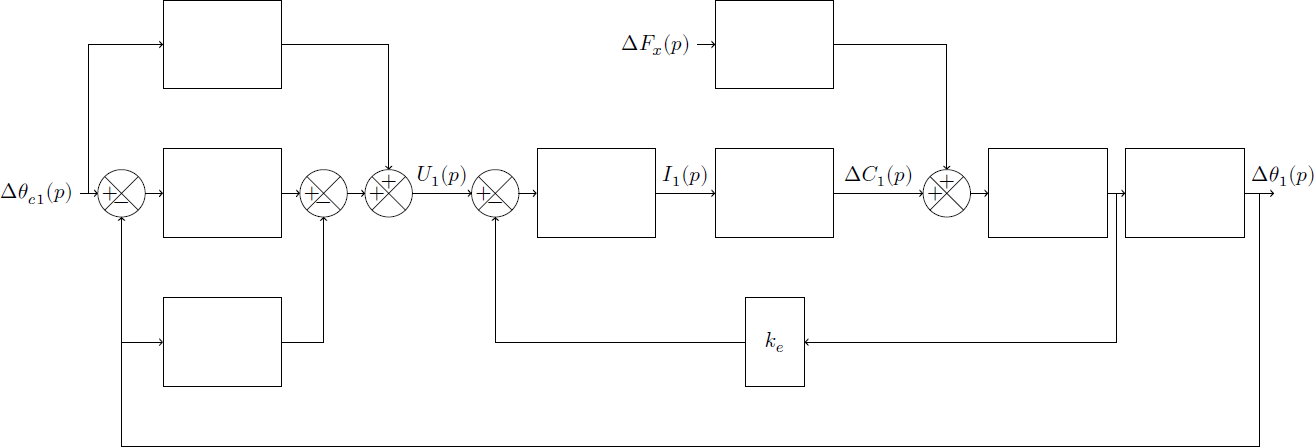
\includegraphics[width=\linewidth]{images/fig_03}
%\textit{Schéma-blocs de l'asservissement du dosseret \label{fig6}}
\end{center}

%\begin{center}
%\includegraphics[width=\linewidth]{images/schema_bloc.jpg}
%
%\textit{Schéma-blocs de l'asservissement du dosseret \label{fig6}}
%\end{center}

\end{document}

\subparagraph{}\textit{}
\ifprof
\begin{corrige}
\end{corrige}
\else
\fi

\begin{center}
\includegraphics[width=\linewidth]{images/}
%\textit{}
\end{center}
\begin{center}
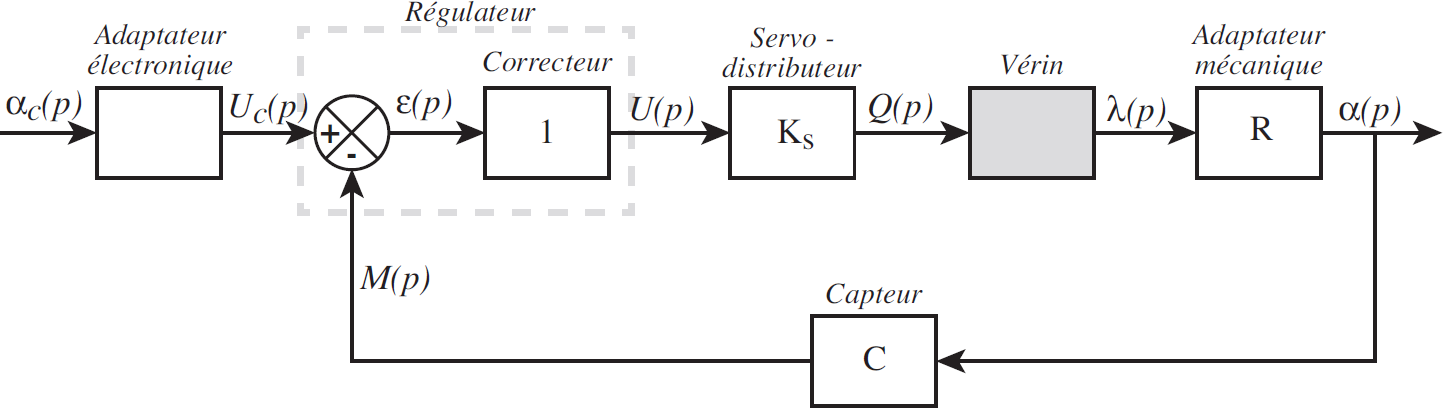
\includegraphics[width=\linewidth]{images/fig_04}
%\textit{}
\end{center}

